\documentclass[b5paper,opensource]{./template/qyxf-book}

% 这里可以自定义一些命令
\newcommand{\di}[1]{\mathrm{d}#1}
\newcommand{\p}[2]{\frac{\partial #1}{\partial #2}}
\newcommand{\pp}[2]{\frac{\partial ^2 #1}{\partial #2 ^2}}
\newcommand{\dy}[2]{\frac{\di{#1}}{\di{#2}}}
\newcommand{\ddy}[2]{\frac{\mathrm{d} ^2 #1}{\mathrm{d} #2 ^2}}
\newcommand{\zbj}[4]
{
	\draw (0,0) node[below left] {$ O $};
	\draw [->] (#1,0) -- (#2,0) node[right] {$ x $};
	\draw [->] (0,#3) -- (0,#4) node[right] {$ y $};
}


\begin{document}

\chapter{质点运动学和牛顿运动定律}
\section{选择题}

\exercise{1}A

\solve
如图1.1,对M,在x方向上:
\begin{figure}[htbp]
	\centering
	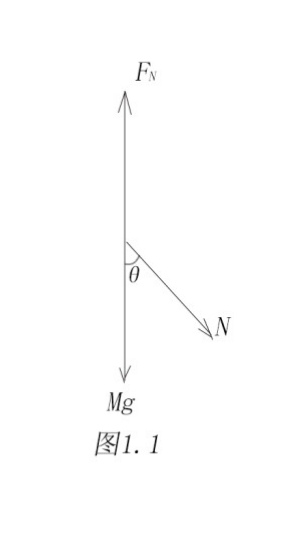
\includegraphics[width=0.3\textwidth]{Chp1_illus1.png}
	\quad
	\centering
	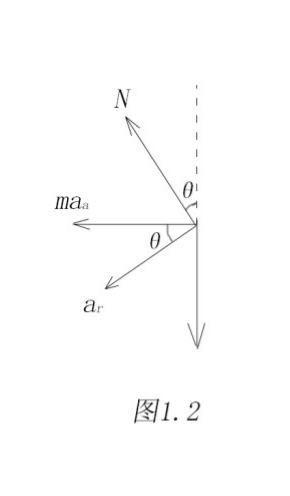
\includegraphics[width=0.3\textwidth]{Chp1_illus2.png}
\end{figure}
\begin{gather}
	N\sin\theta=Ma_e\text{(M对地)}
\end{gather}
如图1.2,对m,以M为参考系,m受一惯性力,合加速度沿二者接触面。
沿x,y方向分解:
\begin{gather}
	mg-N\cos\theta=ma_r\sin\theta\\
	ma_e+N\sin\theta=ma_r\cos\theta
\end{gather}
式(1.1)代入式(1.2),与式(1.3)联立解得:
\[
	a_r=\dfrac{(M+m)g\sin\theta}{M+m{\sin^2\theta}}
\]

\exercise{2}B

\solve
如图1.3,$u=v\cos\theta$,v不变而$\theta$增大,需要u减小。\\
\begin{figure}[htbp]
	\centering
	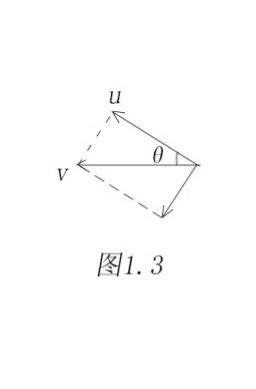
\includegraphics[width=0.3\textwidth]{Chp1_illus3.png}
	%\caption{}
\end{figure}

\exercise{3}A

\solve
匀速圆周运动的速度、加速度(受力)均是大小不变、方向时刻变化。
注意一个矢量为常量包括大小和方向两个方面。否则就是变化的量。

\exercise{4}B

\solve
以前面的货车为参考系,货车静止,火车速率为$v_1-v_2$,加速度为$a$(反向),那么火车最多前进$s=\dfrac{{(v_1-v_2)}^2}{2a}$。要求$d>s$,故选B。或采用地面参考系的追逐问题法,计算从$v_1\text{减速到}v_2$两车走过的距离之差:$s=\dfrac{{v_1}^2-{v_2}^2}{2a}-v_2\cdot \dfrac{v_1-v_2}{a}=\dfrac{{(v_1-v_2)}^2}{2a}$

\exercise{5}C

\solve
两次求导得:$a=30t$,不等于常数而大于零。

\exercise{6}B

\solve
求导得:$v=8t-6t^2,a=8-12t$

令$y=0\Rightarrow t=0\text{(舍去)或}2$s,代入得结果。

\exercise{7}B

\solve
物体做匀加速直线运动。
\begin{gather*}
	s=\dfrac{b}{\cos\alpha},a=g\sin\alpha\\
	t=\sqrt{\dfrac{2s}{a}}=\sqrt{\dfrac{4b}{g\sin(2\alpha)}}
\end{gather*}

$t$最小时,$\sin(2\alpha)$最大,$\alpha=45^\circ$。

\exercise{8}B

\solve
类比从静止出发的匀加速直线运动。$\dfrac{1}{2}\beta t^2=2\pi$

\exercise{9}B

\solve
曲线的定义:“动点运动方向连续变化的轨迹”\footnote{来源:汉典网http://www.zdic.net/c/2/111/299079.htm}。A,C的反例:匀速圆周运动。做曲线运动的物体一定有加速度。

\exercise{10}D

\solve
反例:平抛运动

\section{填空题}

\exercise{11}0\qquad2g

\solve
设A、B质量为m。抽走C之前,弹簧中的弹力大小为mg。撤去C时,弹簧长度未突变,弹力不变,A受合力为0;支持力则消失。

故$a_A=0$,$a_B=\dfrac{mg+mg}{m}=2g$,竖直向下。

\exercise{12}$\dfrac{25}{12}\pi$ rad/$\textrm{s}^2$ \qquad$\dfrac{24}{5} \textrm{s}$

\solve
简单公式应用。
\begin{gather*}
	\text{}\theta=60\times2\pi=120\pi\\
	\beta=\dfrac{\omega_2^2-\omega_1^2}{2\theta}=\dfrac{25}{12}\pi\ rad/s^2\\
	\Delta t=\dfrac{\omega_2-\omega_1}{\beta}=\dfrac{24}{5}s
\end{gather*}

\exercise{13}$m(\sin\theta-\omega^2l\sin\theta\cos\theta)$

\solve
\begin{figure}[htbp]
	\centering
	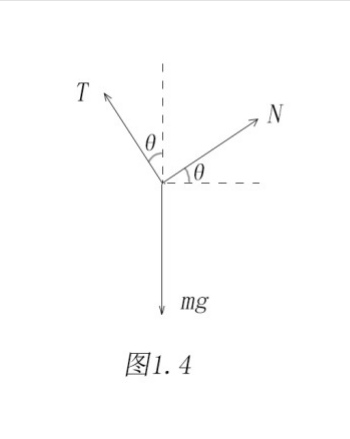
\includegraphics[width=0.5\textwidth]{Chp1_illus4.png}
	%\caption{}
\end{figure}
如图1.4,在x,y方向上分解受力,得:
\begin{gather*}		
	T\sin\theta-N\cos\theta=m\omega^2l\sin\theta\\
	T\cos\theta+N\sin\theta=mg
\end{gather*}
联立可解得$T$、$N$的大小。

\exercise{14}$2\sqrt{\dfrac{r}{g}}$ \qquad $2\sqrt{\dfrac{r}{g}}$

\solve
设弦与PC的夹角为$\theta$,则有:
\begin{gather*}
	s=2r\cos\theta,a=g\cos\theta\\
	t=\sqrt{\dfrac{2s}{a}}=2\sqrt{\dfrac{r}{g}}
\end{gather*}
结果与$\theta$无关。


\exercise{15}$4\sqrt{5}\textrm{m/s}$ \qquad $16\textrm{m/s}^2$

\solve
抛物线的切线方向即为质点的速度方向,且$x=v_xt$。
\[
	\dfrac{v_y}{v_x}=\dy{y}{x}=x\Rightarrow v_y=4x=16t
\]
$x=2$m时,$t=0.5$s,则:
\begin{gather*}
	v_y=8\textrm{m/s}\\
	v=\sqrt{{v_x}^2+{v_y}^2}=4\sqrt{5}\mathrm{m/s}
\end{gather*}
$v_x$不变,故:
\[
	a=a_y=\dy{v_y}{t}=16\textrm{m/s}^2
\]

\exercise{16}长度、质量、时间

\solve
见课本。

\exercise{17}3\quad 3\quad 6

\solve
x分别对t求一阶、两阶导即是v、a,由图像即可判断其正负号。

\exercise{18}$y={(x+5)}^3$

\solve 
由题,$x=2t-5\Rightarrow 2t=x+5$。

代入$y=8t^3={(2t)}^3$,消去t即可。

\exercise{19}$\dfrac{1}{2}g$\qquad 竖直向下

\solve
初始时受力平衡,两根弹簧上力均为$\dfrac{1}{2}mg$;
一根断掉后,向上的力减半,则小球受的合力是$\dfrac{1}{2}mg$,竖直向下。

\exercise{20}$9$m/s

\solve
\begin{align*}
	\text{(SI)} x=3t+6t^2-2t^3&\xrightarrow{\text{求导}}v=3+12t-6t^2\\
	&\xrightarrow{\text{求导}}a=12-12t
\end{align*}
令$a=0$,解得
\[
	t=1\xrightarrow{\text{代入得}} v(1)=9\mathrm{m/s}
\]

\section{计算题}

\exercise{21}

\solve
由图知:
\begin{gather*}
	\tan\alpha=\dfrac{|\vec{a}_n|}{|\vec{a}_\tau|}=\dfrac{\frac{v^2}{R}}{\dy{v}{t}}\\
	\frac{\di{v}}{v^2}=\frac{\di{t}}{R\tan\alpha}
\end{gather*}
积分得:
\[
	-\frac{1}{v}=\frac{1}{R\tan\alpha}t+C
\]
代入$t=0,v=v_0$:
\[
	C=-\dfrac{1}{v_0}\Rightarrow -\frac{1}{v}=\frac{t}{R\tan\alpha}-\dfrac{1}{v_0}
\]
所以:
\[
	v=\frac{v_0R\tan\alpha}{R\tan\alpha-v_0t}
\]

\exercise{22}

\solve
\begin{gather*}
	\vec{v}=\dy{s}{t}\vec{\tau}=(c+2dt)\vec{\tau}\\  
	\vec{a}_n=\frac{v^2}{R}\vec{n}=\frac{(c+2dt)^2}{R}\vec{n}\\
	\vec{a}_\tau=\dy{v}{t}\vec{\tau}=2d\vec{\tau}
\end{gather*}
令$|\vec{a}_n|=|\vec{a}_\tau|$,则
\begin{gather*}
	\frac{(c+2dt)^2}{R}=2d\\
	t=t_1=\frac{\sqrt{2dR}-c}{2d}\left(t_2=\frac{-\sqrt{2dR}-c}{2d}<0\text{,舍去}\right)
\end{gather*}
$\therefore$要使$t\geqslant0$,条件为$\sqrt{2dR}-c\geqslant0$,即$2dR\geqslant c^2$。

\exercise{23}

\solve
\[
	-kx=a=\dy{v}{t}=\dy{v}{x}\cdot \dy{x}{t}=\dy{v}{x}\cdot v
\]
分离变量,积分得:
\[
	-\dfrac{1}{2}kx^2+C_1=\dfrac{1}{2}v^2
\]
令$C=2C_1$,则$-kx^2+C=v^2$。
代入$x=x_0,v=v_0$,得:
\[
	C=kx_0^2+v_0^2
\]
整理得:
\[
	v=\pm\sqrt{kx_0^2+v_0^2-kx^2}
\]

\exercise{24}

\solve

(1)

$\dy{x}{t}=v=10\left(1-\dfrac{t}{5}\right)=-2t+10$

$x=-t^2+10t+c$

代入$t=0,x=0$得:$x=-t^2+10t$

代入$t=10s$得$x=0$。

$\therefore$坐标为$0$

(2)
令$x=10m$,则$t^2-10t+10=0$。

$\therefore\ t=5\pm\sqrt{15}$ s

令$x=-10m$,则$t^2-10t+10=0$

$\therefore\ t=5+\sqrt{35}(5-\sqrt{35}<0,\text{舍去})$

$\therefore$时刻为$5-\sqrt{15}\ \textrm{s},5+\sqrt{15}\ \textrm{s}\text{或}5+\sqrt{35}\ \textrm{s}$

(3)
令$v=0$,则$t=\ 5s$。此时质点运动方向改变。

$\therefore t\in[0,5]$时,$s=x=-t^2+10t$

$t\in[5,+\infty)$时,
\begin{align*}
	s&=s(5)+[s(5)-x]\\
	&=25+[25-(-t^2+10t)]\\
	&=t^2-10t+50
\end{align*}

$\therefore\ s=
\begin{cases}
-t^2+10t,&t\in[0,5)\\
t^2-10t+50,&t\in[5,+\infty)
\end{cases}$

\end{document}
